\documentclass[a4paper,abstract=true]{scrartcl}

% ----- Encoding & Fonts
\usepackage[T1]{fontenc}
\usepackage[utf8]{inputenc}
\usepackage{lmodern}
\usepackage{microtype}


\usepackage[english]{babel}

% ----- Zitate/Anführungen
\usepackage{csquotes}

% ----- Grafik & Layout
\usepackage{graphicx}
\usepackage{subcaption}
\usepackage{booktabs}
\usepackage{longtable}
\usepackage{tabularx,ragged2e}
\newcolumntype{Y}{>{\RaggedRight\arraybackslash}X}

% ----- URL/Links
\usepackage[hyphens,spaces,obeyspaces]{url}
\usepackage[hidelinks]{hyperref}
\usepackage{orcidlink}

\usepackage{cleveref}

% ----- biblatex (nach babel, csquotes, hyperref)
\usepackage[backend=biber,style=acmnumeric,doi=true,url=true]{biblatex}
\addbibresource{helios_prototype.bib}




% ----- Boxen, Listings etc.
\usepackage[most]{tcolorbox}
\newtcolorbox{summarybox}{
    enhanced, breakable, sharp corners,
    boxrule=0.3pt, colback=white, colframe=black!40,
    coltitle=black, fonttitle=\bfseries,
    toptitle=2mm, bottomtitle=2mm, colbacktitle=white,
}
\usepackage{listings}
\usepackage{xcolor}
\definecolor{codegray}{gray}{0.9}
\definecolor{commentgreen}{rgb}{0,0.6,0}
\definecolor{keywordblue}{rgb}{0.2,0.2,0.8}

\lstdefinestyle{c++style}{
    backgroundcolor=\color{white},
    commentstyle=\color{commentgreen}\itshape,
    keywordstyle=\color{keywordblue}\bfseries,
    numberstyle=\tiny\color{gray},
    stringstyle=\color{red},
    basicstyle=\ttfamily\small,
    breaklines=true,
    captionpos=b,
    keepspaces=true,
    numbers=left,
    numbersep=5pt,
    showspaces=false, showstringspaces=false, showtabs=false,
    tabsize=2, language=C++
}

% ----- Anhang
% Entweder KOMA intern nutzen (empfohlen) ODER appendix-Paket.
% Wenn du das Paket behalten willst, okay:
\usepackage[titletoc,title,page,header]{appendix}
\renewcommand{\appendixname}{Anhang}
\renewcommand{\appendixtocname}{Anhänge}
\renewcommand{\appendixpagename}{Anhänge}

% ----- Sonstiges
\usepackage{dirtree}
\renewcommand*\DTstyle{\ttfamily}

% Silbentrennungen
\hyphenation{
    Ren-de-ring-Back-end
    Game-Loop
    Smart-Poin-ter
    Kol-li-sions-be-hand-lung
    er-strek-ken
}


\begin{document}

    \title{\textbf{helios: Design and prototypical implementation of a C++ game framework}}
    \subject{Technical Report}

    \author{%
        Thorsten Suckow-Homberg%
        \thanks{%
            \href{mailto:thorsten@suckow-homberg.de}{thorsten@suckow-homberg.de}, Trier University of Applied Sciences, Department of Computer Science. DOI: 10.5281/zenodo.xxxxxxx;
            Licensed under \href{https://creativecommons.org/licenses/by/4.0/}{CC BY 4.0}%
        }%
    }

    \date{November 2025}

    \maketitle





    \begin{abstract}
    Wir stellen \textit{helios} vor, einen in C++ entwickelten Prototyp eines Game Frameworks zur Umsetzung eines \textit{Geometry Wars}-Klons.
    Wir beschreiben den grundlegenden Aufbau des Frameworks und gehen auf die Funktionalitäten vorhandener Module ein.
    Architektur- und Designentscheidungen werden begründet, ebenso die Herausforderungen, die sich während der Entwicklung ergeben haben.
    Abschließend geben wir einen Ausblick, in welchen Bereichen wir im weiteren Verlauf der Entwicklung die größten Änderungen erwarten.
\end{abstract}

\section{Introduction}

We are developing a \textit{Geometry Wars}\footnote{See~\cite[]{WikipediaGeometryWars}} clone in~C++.
In doing so, we partly base our implementation on a widely used game engine architecture described by Gregory in~\cite[]{Gre19}, while deliberately reducing the number of abstraction layers and omitting systems such as tooling, sound, and scripting (cf.~\cite[Figure~1.16, p.~39]{Gre19}).
The technical foundation therefore resembles a framework rather than a complete engine.
The actual game - conceived as a \textit{black box}~\cite[]{RB88} - is intended to use the framework's interfaces to access the required hardware and other subsystems.

\begin{figure}[tbp]
    \centering
    \includegraphics[width=0.5\columnwidth]{img/helios_logo}
    \caption{The \textit{helios} project logo. (Source: own representation)}
    \label{fig:helios_logo}
\end{figure}

The following sections present the architecture of the framework, referred to as \textbf{helios}\footnote{
    Helios, who “looks sharply about with shining eyes” (\textit{Homers Ilias}, Gesang~14, own translation), is the sun god in Greek mythology.
}, and discuss its prototypical development stage.
The software is being created within an agile \textit{Tracer Bullet Development} process~\cite[pp.~50~f.]{TH20}, which allows the entire system to be adapted at short notice if necessary.
From this, the architectural requirements are derived.
The project data and objectives are presented separately in Section~\ref{sec:projectdata}.

Furthermore, we discuss challenges and difficulties encountered during implementation.
These arise, among other factors, from the fact that the software - to be developed within a comparatively short time frame - is evaluated not only according to objective measures (such as the number of defects, software design choices, or object coupling), but also according to subjective criteria~\cite[385]{Bal08}.
Although there are no plans to classify the finished product according to usability quality characteristics such as ISO/IEC~9126\footnote{Usability quality according to ISO/IEC~9126,~\cite[466]{Bal08}; see also studies and investigations in~\cite[]{AZMK17} and~\cite[]{Ber10}.}, the result should not only be technically sound but also pleasant to use.
We summarize this user experience in general terms using the expression \textit{game feel}~\cite[]{Swi08}, established in contemporary game development.

\section{Project Data and Goals}\label{sec:projectdata}

The goal of this project is to create a stable prototype of the twin-stick shooter\footnote{
    For genre classification, see also~\cite[]{GameDeveloper}.
} \textit{Geometry Wars} (see Figure~\ref{fig:geometry_wars}) using the C++23 programming language and the OpenGL API~\cite[]{OpenGLHomepage}.\\

\begin{figure}[tbp]
    \centering
    \includegraphics[width=1\columnwidth]{img/geometry_wars}
    \caption{\textit{Geometry Wars} first appeared in 2003 as an Easter egg in the game \textit{Project Gotham Racing 2} (Microsoft Game Studios). Due to its great popularity, several sequels were released, most recently in 2016 with \textit{Geometry Wars 3: Dimensions Evolved} (Activision). (Source: Activision Publishing, Inc.)}
    \label{fig:geometry_wars}
\end{figure}

The following features were agreed upon for implementation:

\begin{itemize}
    \itemsep0.5em
    \item Playable level (2D grid)
    \item Time attack mode with a duration of 3 minutes
    \item High score system
    \item Controller support
    \item Stable frame rate of at least 60 FPS with simultaneous display of over one hundred enemies and objects
    \item Three enemy types with simple AI (``spawn and chase``)
    \item Enhancement of the game feel through graphical effects
    \item Compilable and executable under Windows~11
\end{itemize}

While some criteria are specifically measurable (e.g., frame rate), other requirements are deliberately vague (e.g., game feel) and underscore the exploratory nature of the project.
Formal requirements engineering is therefore not part of this work, especially since the original game on which the implementation is based also serves as a reference and benchmark.

The learning process itself is considered a key objective of this project; no formal metrics are used for its evaluation.
Instead, the experiences and results obtained are documented in writing, and the present report will serve as a critical reflection of them at the end of the project.


Against this background, the approach can be regarded as a form of dynamic requirements engineering ``with significantly greater degrees of freedom``~\cite[60]{MRP21} (own translation).
The aforementioned \textit{Tracer Bullet Development} process, which primarily provides a platform for integration, corresponds to the prototype referred to by Pflug et~al. as a ``living lab``, which is further developed using agile methods (\textit{ibid., p.~61}), allowing for the contribution of original creative ideas.\footnote{
    In~\cite[]{KMS14}, Kasurinen et~al.\ explore whether requirements management, which is rooted in engineering, has a place in game development, a field strongly influenced by creative processes. They show that some requirements are consciously derived through \textit{user testing}. Accordingly, games user research has become an important branch of the games industry that helps developers understand and improve the player experience (\cite[p.~26]{Zam18}). Further discussions regarding software engineering in game development can be found in Kanode and Haddad~\cite[]{KH09}.
}

\subsection{Schedule}

The schedule and associated milestones are presented in Table~\ref{tab:schedule}.
The timeline serves as a guideline for implementation; the sequential listing does not imply a waterfall model.

\setlength{\tabcolsep}{8pt}
\begin{table}[t]
    \centering
    {\renewcommand{\arraystretch}{1.2}%
        \begin{tabularx}{\textwidth}{@{} l l Y @{}}
            \toprule
            \textbf{Milestone} & \textbf{Date} & \textbf{Content} \\
            \midrule
            \texttt{milestone\_1} & 2025-10-20 &
            Provision of the application layer, including implementation of the event system,
            the input manager, and connection to the low-level API subsystem. \\
            \texttt{milestone\_2} & 2025-11-17 &
            Provision of the rendering engine; initial design of the playing field, including display of the player's ship. \\
            \texttt{milestone\_3} & 2025-12-22 &
            Implementation of physics and player input for ship control; fire mechanics. \\
            \texttt{milestone\_4} & 2026-01-19 &
            Implementation of the core game rules and mechanics; playable prototype. \\
            \texttt{milestone\_5} & 2026-02-09 &
            Provision of the prototype; fine-tuning. \\
            \texttt{milestone\_6} & 2026-03-16 &
            Submission of documentation and presentation of the project. \\
            \bottomrule
        \end{tabularx}}
    \caption{Planned milestones for the implementation of the \textit{Geometry Wars} clone.
    At the time of publication of this document, the first milestone has been completed: \textit{helios} already provides simple window management, rudimentary input processing, a logging system, and a functional rendering layer with a connection to the OpenGL API.}
    \label{tab:schedule}
\end{table}

\noindent
Since the game concept to be implemented is already defined, there is no need for an exploratory prototype phase.
The current stage of development can be classified as the \textit{hard-architecture design} phase, following Rollings and Morris~\cite[pp.~628-630]{RM04}.

The project is published under the MIT license on GitHub, with both the source code and the issue tracker publicly accessible~\cite[]{heliosgithub}.

\section{Project Structure}

We present the structure of the project and the associated toolchain.
We also briefly introduce the contents of the individual directories.\\

The top level of the \textit{helios} directory structure provides access to tests, executable sample programs, benchmarks, documentation, and source files.
The chosen structure follows the conventions for C++ projects defined by the \textit{Pitchfork} project~\cite[]{Pitchfork}.
The directory names are self-explanatory and are shown in Figure~\ref{fig:directory_structure}.

\begin{figure}[htbp]
    \setlength{\DTbaselineskip}{18pt}
    \dirtree{%
        .1 ./.
        .2 benchmarks/.
        .2 docs/.
        .2 examples/.
        .2 include/.
        .2 src/.
        .2 tests/.
    }
    \caption{Project directory of \textit{helios} (excerpt).}
    \label{fig:directory_structure}
\end{figure}

The project comprises several build stages to compile the source files and generate the tests and example programs.
For automation, we use \texttt{CMake}~\cite[]{CMake}, which also allows us to perform simple dependency management.
The third-party libraries (TPLs) required for development (including \texttt{glfw}~\cite[]{glfwHomepage} and \texttt{glad}~\cite[]{gladgithub}) can thus be fetched directly from external sources, statically compiled, and integrated (see Listing~\ref{lst:cmake}).
This approach enables us to automate the project’s preconfiguration and avoid manual (and often error-prone~\cite[]{FG22}) integration of TPLs.

\vspace{4mm}
\begin{lstlisting}[style=c++style,
    caption={Excerpt from helios' CMakeLists.txt.
    This section declares and fetches GLFW v3.4 and GLAD v2.0.8 via \texttt{FetchContent} from the respective GitHub repositories (URLs omitted for clarity).
    Subsequently, a GLAD loader for OpenGL 4.6 is created as a static library.},
    label=lst:cmake]
...
FetchContent_Declare(glfw
    GIT_REPOSITORY [url]
    GIT_TAG        3.4
)

FetchContent_Declare(glad
    GIT_REPOSITORY [url]
    GIT_TAG        v2.0.8
    SOURCE_SUBDIR cmake
)

FetchContent_MakeAvailable(glfw glad)

# GLAD v2: Core GL 4.6
glad_add_library(
    glad_gl_core_46 STATIC REPRODUCIBLE LOADER API 
    gl:core=4.6
)
...
\end{lstlisting}

\subsection{Directory Contents}

In the following, we present the main directories in alphabetical order and briefly discuss their contents.

\subsection*{\texttt{/benchmarks}}

For benchmarking individual functions, \textit{helios} uses \textit{Google Benchmark}~\cite[]{googlebenchmarkgithub}.
Currently, there are benchmarks for mathematical types and functions.
We use these to compare our implementations with those of \texttt{glm}~\cite[]{glmGithub}, which serves as a reference.
This allows us to identify potential bottlenecks in the \textit{Game Loop} at an early stage, for example in operations involving affine transformation matrices.
Further benchmarks - measuring the performance of selected functions in the \textit{Rendering Pipeline} or \textit{Application Stage}~\cite[687]{Gre19} (e.g., during \textit{Culling}) - are planned.

\setlength{\tabcolsep}{8pt}
\begin{table}[t]
    \centering
    {\renewcommand{\arraystretch}{1.2}%
        \begin{tabular}{lrrr}
            \hline
            \textbf{Benchmark} & \textbf{Time} & \textbf{CPU} & \textbf{Iterations} \\
            \hline
            BM\_mat4Constructor/real\_time & 5.81 ns & 5.85 ns & 106,874,145 \\
            BM\_mat4Multiply/real\_time    & 175 ns  & 168 ns  & 3,896,895 \\
            \hline\\
        \end{tabular}}
    \caption{Sample output of benchmark results based on our custom \texttt{mat4} implementation.}
    \label{tab:mat4-benchmark}
\end{table}

No evaluation of alternative benchmarking frameworks was conducted; the choice was based on popularity and community recommendations.

\subsection*{\texttt{/docs}}

In addition to formal documentation\footnote{Such as the \LaTeX\ source code of this document.},
this directory contains API documentation generated from the source files using \texttt{doxygen}~\cite[]{Doxygen}.
A key advantage of \texttt{doxygen} is its ability to export to multiple formats.
This allows us to generate HTML or XML documentation and integrate it into the \textit{helios} project website~\cite[]{helios} via a dedicated build step.

A formal evaluation of documentation tools was not performed.
The selection was guided by ease of integration and widespread adoption.
We also consider the extensive range of output formats (including PDF and Markdown) beneficial for maintaining project documentation.

\subsection*{\texttt{/tests}}

For unit testing, \textit{helios} employs \textit{Google Test}~\cite[]{googletestgithub}.
To increase development speed, especially during the early and potentially unstable project phase, we initially decided against pursuing high test coverage.
Current tests therefore focus on mathematical functions - for instance, validating transformations within the scene graph.
\textit{helios} uses \texttt{glm} as a test oracle~\cite[pp.~917-919]{Bin99} for comparison purposes.\footnote{
    Alternatively, \texttt{glm} can be regarded as a \textit{baseline} against which \textit{helios} functions (as a \textit{delta version}) are compared in regression tests.
    We acknowledge that any errors in \texttt{glm} would propagate to \textit{helios}; however, given the maturity of the \textit{glm} project, this risk is considered minimal.}

As with benchmarking, no formal evaluation of unit testing frameworks was conducted.
The decision was based on popularity and recommendations.

\subsection*{\texttt{/examples}}

This directory contains example programs that demonstrate the individual functionalities of the framework.
During development, these programs help define functionalities in a \textit{top-down approach} and refine them iteratively~\cite[]{Wir71}.
This approach allows us to focus on the required interfaces of individual subsystems without getting lost in implementation details that can be added in later iterations.

\begin{figure}[!h]
    \centering
    \includegraphics[width=1\columnwidth]{img/cube_example}
    \caption{Screenshot of the \texttt{simple\_cube\_rendering} demo, used in a top-down approach to incrementally implement the functionality defined in the first milestone. (Source: own recording)}
    \label{fig:simple-cube-rendering-demo}
\end{figure}

\subsection*{\texttt{/include, /src}}

With C++23, \textit{helios} implements its classes and functions entirely through Module Interface and Implementation Units~\cite[pp.~211-213]{Str24}.
These are stored in \texttt{/include} and \texttt{/src}, respectively.
Modules not divided into Interface and Implementation Units reside exclusively in \texttt{/include} as ``header-only`` components.
These include classes such as \texttt{helios::math::vec3}, which represents a three-dimensional vector type whose functions are predominantly declared as \texttt{constexpr}\footnote{
    The \texttt{constexpr} keyword allows expressions to be evaluated at compile time, requiring their complete definition at translation time~\cite[p.~330]{Gre24}.}.
The directories are further subdivided into \texttt{ext} and \texttt{helios}:
\begin{itemize}
    \itemsep0.5em
    \item \texttt{ext} contains platform-specific implementations of interfaces contractually defined by the \textit{helios} framework (hardware-related window and application abstractions, as well as rendering pipeline specifics).
    \item \texttt{helios} contains the actual framework code.
\end{itemize}

\section{Architecture}
In the following, we describe the architecture of helios, which is currently designed as shown in Figure ~\ref{fig:hardarchitecture}: helios acts as an intermediary layer between the game as a real-time data model~\cite[525]{Gre19} and the technical infrastructure.
The framework visualizes the game state and transmits input data to the game as control commands.

\begin{figure}[!h]
    \centering
    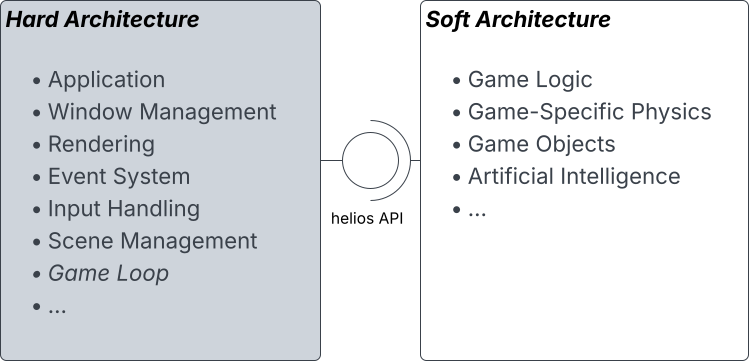
\includegraphics[width=1\columnwidth]{img/hardarchitecture_en.svg}
    \caption{Division of the architecture of the helios framework into \textit{hard} and \textit{soft architecture} according to Rollings and Morris~\cite[612 ff.]{RM04}. The ball/socket notation illustrates that helios provides interfaces that can be used by any game. (Source: own representation)}

    \label{fig:hardarchitecture}
\end{figure}

Figure~\ref{fig:package_diagram} shows a more detailed view of the modules and selected components.
The directory structure of helios reflects the structure of its core functionalities.
In the sense of \textit{Evans}, this is crucial for high cohesion: The directory names communicate the functionalities they contain~\cite[180 f.]{Eva03}.
Within the modules, there is a further subdivision into layers (such as \texttt{controller}), which is referred to as ``package-by-feature and -by-layer``.


\begin{figure*}[t]
    \centering
    \makebox[\textwidth][c]{% Box is text-width, content may extend beyond
        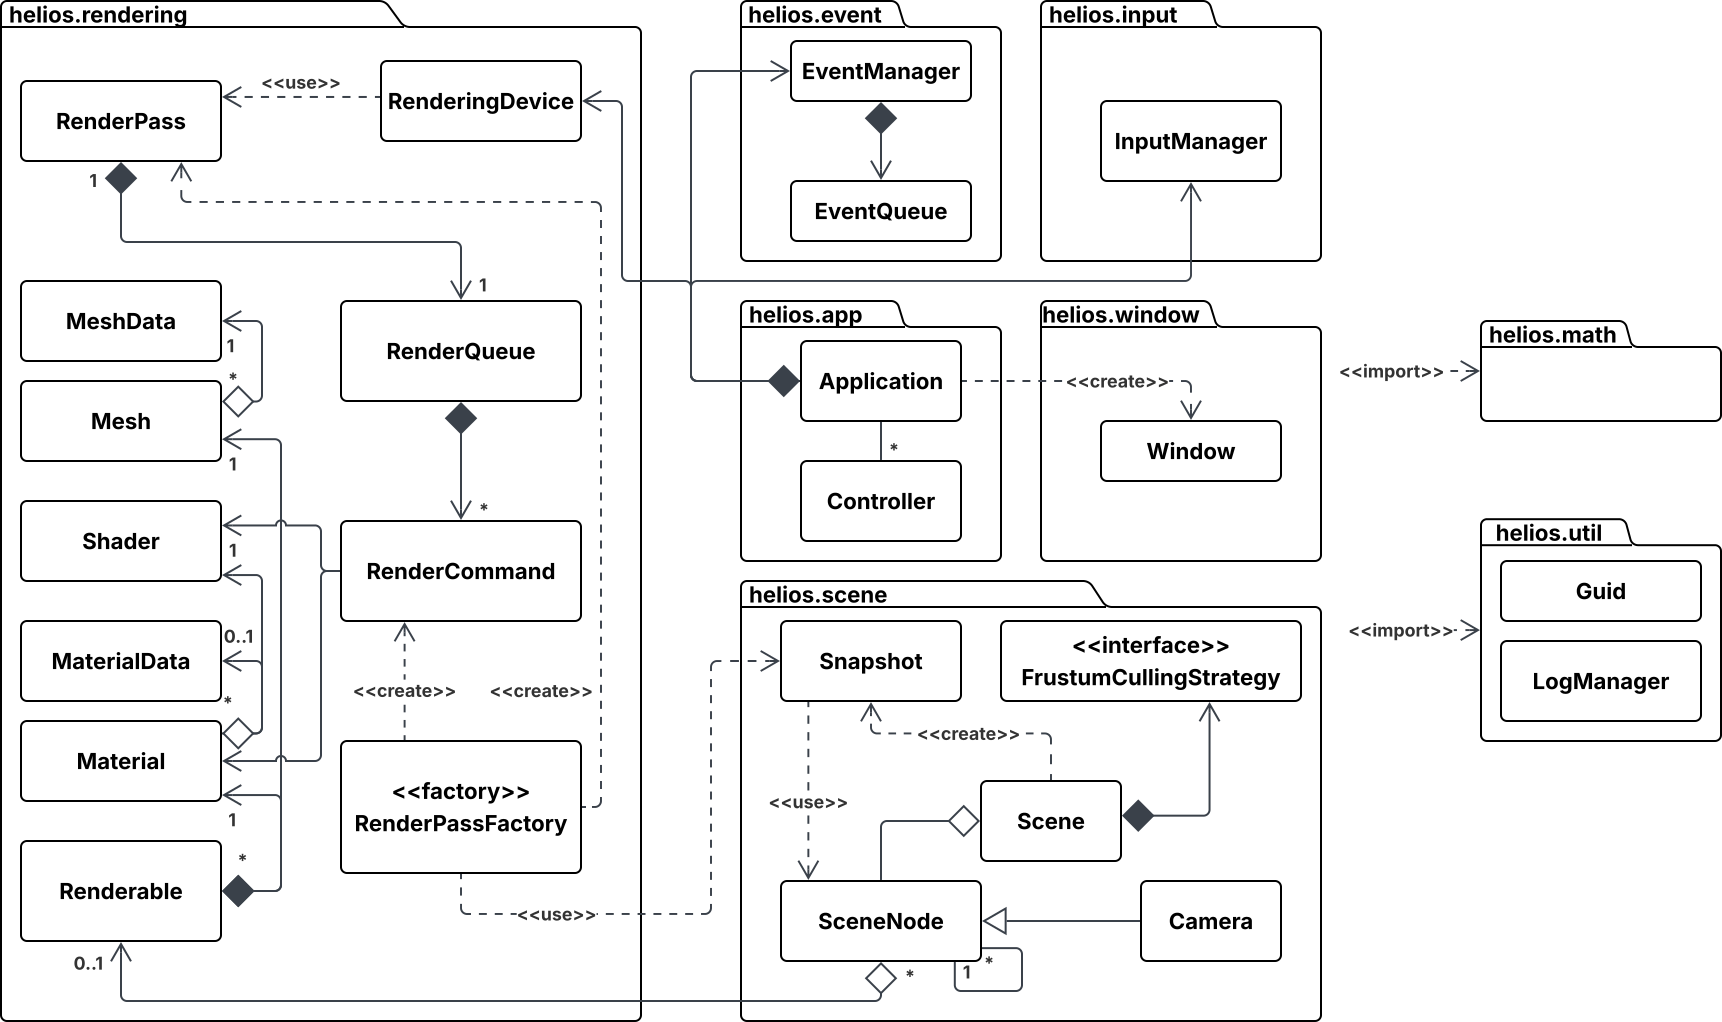
\includegraphics[width=1\textwidth]{img/package_diagram.svg}% \linewidth == column width
    }
    \caption{Structure of the helios framework and relationship between some selected components. The modules are structured according to a ``by-feature, by-layer`` concept, in which features are divided internally into functional layers. (Source: own representation)}

    \label{fig:package_diagram}

\end{figure*}


\subsection*{\texttt{app}: Application layer}
The central control unit of the application or game is the \texttt{Application} class, which provides the event system, input processing, and window management, and initializes the rendering backend - represented by \texttt{RenderDevice}.
helios also supports dynamic addition of application controllers~\cite[379] {Fow03} for defining isolated, event-based control logic, such as behavior during a window resize\footnote{
    The application controllers were originally introduced to abstract ``framebuffer resize`` events from the rendering backend.
}.

\subsection*{\texttt{input}: Input processing}
The \texttt{InputManager} orchestrates input processing.
It is managed exclusively by the application and bound to the active window.
A specialized \texttt{InputAdapter} abstracts the input events provided by the TPLs and translates them for the \texttt{InputManager}.
At the beginning of the game loop, active input events are polled (\texttt{InputManager::poll()}). Events are queried using methods such as \texttt{InputManager::isKeyPressed()}.

\subsection*{\texttt{event}: Event processing}
Events can be written to an \texttt{EventQueue} (``\textit{post}``) via the \texttt{EventManager}.
Interested observers (\textit{Observer}) can register with the \texttt{EventManager} via callbacks using \texttt{subscribe}~\cite[293 ff.]{GHJV94}.
The method \texttt{EventManager::dispatchAll()} informs the observers about existing events.

\subsection*{\texttt{window}: Window class}
The \texttt{Window} class provides interfaces for controlling the application window, querying window events, and instructing \textit{buffer swapping}.


\subsection*{\texttt{math}: Mathematical types and operations}
This module provides trigonometric functions and representatives for data types anchored in linear algebra, such as vectors and matrices, in the namespace \texttt{helios::math}.
It also supports operations for linear and affine transformations, thereby implementing the coordinate space change commonly used in 3D computer graphics\footnote{
    After projection, the coordinates are available in the so-called clip space.
    Typically, the rendering backend uses perspective division to convert these coordinates into NDC (\textit{Normalized Device Coordinates}) relevant for the rasterizer~\cite[18]{AHHP+18}.
}:

\[
    \text{Model}\rightarrow\text{World}\rightarrow\text{View}\rightarrow\text{Projection}
\]

\noindent

The interfaces are based on popular libraries such as the aforementioned \texttt{glm} for their method signatures.

\subsection*{\texttt{scene}: Scene graph}
The scene graph \texttt{helios::scene::Scene} follows established implementations from the literature\footnote{See, among others,~\cite[]{She07} and~\cite[]{Gre19}.}.
\texttt{Scene} has an implicit root node that can contain any number of child nodes.
Each \texttt{SceneNode} has a \texttt{Transform} object that describes the model transformation in the local coordinate system.
\texttt{SceneNodes} can be ``renderable``, i.e., they are configured with a \texttt{Renderable}.
However, they can also simply represent a camera (\texttt{helios::scene::Camera})\footnote{
    In this context, other node types usually include (freely positionable) \texttt{LightNodes}, i.e., light sources.
}.
Scene nodes with \texttt{Renderable} are taken into account during \textit{culling}.
The culling procedure is defined abstractly in the purely virtual class \textit{FrustumCullingStrategy}. Specializations are passed to the \texttt{Scene} during instantiation.
In the application stage~\cite[687]{Gre19}, helios creates a \texttt{Snapshot} from a scene and a camera, for which the configured culling strategy collects all \texttt{SceneNode}s located in the camera's visible area.
A single snapshot forms the basis for a \texttt{RenderPass}, which contains the necessary instructions (\texttt{RenderCommand}s) for the actual rendering process.
Listing~\ref{lst:gameloop} shows the sequence of a simple game loop.


\begin{lstlisting}[style=c++style, caption={Implementation of a simple game loop in helios. A \texttt{snapshot} is created from the scene, which serves as the basis for the \texttt{RenderPass}.}, label=lst:gameloop]
while (!win->shouldClose()) {
  app->eventManager().dispatchAll();

inputManager.poll(0.0f);

  if (inputManager.isKeyPressed(Key::ESC)) {
      win->setShouldClose(true);
  }

snapshot   = scene->createSnapshot(*camera);
renderPass = factory.buildRenderPass(
    snapshot
  );

app->renderingDevice().render(renderPass);

  win->swapBuffers();
}
\end{lstlisting}



\subsection*{\texttt{rendering}: Render Pipeline}
The rendering system of helios is divided into different modules, including \texttt{shader} for shader and GLSL\footnote{\textit{OpenGL Shading Language}}-specific code, and \texttt{model} for abstractions of material and mesh data.
\texttt{Renderable}s are representatives of ``renderable`` objects.
They encapsulate information necessary for the rendering process and are modeled as aggregations.
They consist of individually configurable \texttt{Material} and \texttt{Mesh} instances, which in turn share \texttt{MaterialData} and \texttt{MeshData} objects with other instances for easy and resource-efficient reuse~\cite[126]{AHHP+18}.

The information required for a \texttt{RenderPass} is collected as \texttt{RenderCommand} objects in a \texttt{RenderQueue}, which are processed by the actual \texttt{RenderDevice}: \texttt{RenderCommand}s have pointers to the geometry to be rendered (\texttt{Mesh}), the \texttt{Shader} to be used, and data objects in which information about \texttt{Uniform} variables (transformation matrices, etc.) is stored.
The \texttt{RenderDevice} processes a \texttt{RenderPass} using the template methods \texttt{preRender, doRender}, and \texttt{postRender}.


\subsection*{\texttt{util}: Utility classes}
The \texttt{helios::util} module contains non-domain-specific code, such as the \texttt{LogManager} for simple logging functions and a \texttt{Guid} implementation for configuring objects with a global unique identifier (\textit{global unique identifier}).
\section{Discussion of the implementation}

In~\cite[]{PPTD08}, Petrillo et al. describe several causes that lead to \textit{feature creep} in game development.
These include developing proprietary solutions instead of using existing libraries, as well as adding supposedly ``attractive`` features that, considering the YAGNI\footnote{\textit{You Aren't Gonna Need It}~\cite[]{Sch07}} maxim, offer no added value for the actual project goal.
As the authors point out, this puts game development on a par with ``ordinary`` software development, for example in the context of contract work.
If the project also involves a technically unfamiliar domain that has to be implemented within a tight timeframe, a sense of proportion and discipline are essential when implementing functionality.
With helios, we therefore pursue a top-down approach to enable rapid prototyping and, applying the framework concept, to drive forward the step-by-step development and integration of the \textit{Geometry Wars} clone.
In this context, we understand the SOLID\footnote{
    \textbf{S}ingle Responsibility Principle, \textbf{O}pen-Closed Principle, \textbf{L}iskov Substitution Principle, \textbf{I}nterface Segregation Principle, \textbf{D}ependency Inversion Principle
} principles~\cite[]{Mar03} as an indispensable basis for agile software development, as they are closely related to ``clean software design`` and have already proven valuable in the development process to date\footnote{See Cabral et al., who examine SOLID in the machine learning environment in~\cite[]{CKME+24} - an environment they characterize with ``iterative experimentation with data, models, and algorithms.`` They conclude that applying the principles contributes significantly to understanding the source code.
}.

To avoid the emergence of an unstructured, difficult-to-maintain architecture (\textit{Big Ball of Mud}~\cite[]{FY99}), we rely on a clear separation of responsibilities, which is reflected in the project by the various feature layers.
To reduce the degree of coupling between the components involved - and thus improve maintainability and testability - we use \textit{Dependency Injection}~\cite[]{SZ10}, which is mainly implemented through \textit{Constructor Injection}~\cite[]{FowlerDI}.
Since no dedicated DI container is used in the current implementation, the management of dependencies (``\textit{wiring}``) in the actual source code results in additional boilerplate code, which is, however, largely reduced by outsourcing the creation logic to static factory classes.
This particularly benefits the implementations of the sample programs during development, which also serve as test programs.
In other subsystems, factory methods also support the encapsulation of object creation within those entities that are also assigned technical responsibility in terms of business logic~\cite[139 f.]{Eva03}.
In this way, the architecture of helios remains coherent, and dependencies between the layers are kept to the necessary minimum.


We find it rather challenging to deal with modern language features that a proven but also ``traditional`` programming language such as C++ has experienced in recent years - such as the module system or the use of smart pointers: We find ourselves caught between the conflicting demands of applying established C++ idioms~\cite[]{IdiomaticCpp} and proven concepts in a development environment that is predominantly shaped by experience with simpler high-level languages such as Java.
Especially at the beginning of the project, the project structure and namespace identifiers were therefore repeatedly adjusted (see Figure~\ref{fig:code_frequency}).

\begin{figure}[!h]
    \centering
    \includegraphics[width=0.8\columnwidth]{img/code_frequency}

    \caption{Code frequency graph for the helios repository. The changes made to the project structure in the early phase are reflected in the almost symmetrical distribution of added (green) and removed code (red). (Source: GitHub)}
    \label{fig:code_frequency}
\end{figure}

In order to express clear ownership relationships in object management, we refrain from using raw pointers in many places.
Instead, we use the \texttt{unique\_ptr}, \texttt{shared\_ptr}, or \texttt{weak\_ptr} types defined in the standard library, which manage ownership semantics exclusively (through \textit{move} operations) or jointly (through reference counting).
The extent to which the additional CPU instructions resulting from this have a measurable impact on efficiency when building and processing the rendering pipeline must be evaluated at a later date, if necessary\footnote{
A performance comparison is provided, for example, by~\cite[]{Val25}.
}.

We see potential for optimization here, but in the early development phase we have consciously opted for stability and clear semantics.
We accept later refactorings in favor of greater efficiency\footnote{
    These are not necessarily limited to the design of the components or the architecture itself, but can extend to low levels of abstraction - such as ``bare metal`` - to implementations of the math library using SIMD instructions, as provided by \texttt{glm}~\cite[]{glmSimd} (SIMD, short for \textit {single instruction, multiple data}, describes the concept in which a single instruction is executed in parallel on different data).
}, especially since such measures only seem to make sense once the domain has been sufficiently explored, both technically and in terms of the domain\footnote{
    See ``Refactoring toward Deeper Insight``~\cite[]{Eva03}.
}.


The choice of data structures and programming paradigms should also be mentioned at this point: Our object relationships are currently very expressive (\texttt{Snapshot}, \texttt{Renderable}, \texttt{Material}, \texttt{Shader}, etc.), and we have so far been able to avoid excessively deep inheritance hierarchies.
For efficiency reasons, powerful game engines often do not rely entirely on classic OOP paradigms, but instead use a data-oriented approach in performance-critical subsystems, in which flat associations of components according to the \textit{ECS pattern}~\cite[]{RCCK25} can offer significant performance advantages~\cite[]{WWM22}\footnote{See the data-oriented framework \textit{ECS for Unity}~\cite{UnityECS} for Unity. The Unreal Engine also offers \textit{MassEntity}~\cite{UnrealMassEntity}, a ``gameplay-focused framework for data-oriented calculations``}.
This is something we do not consider in this phase of development - but it is something we should keep in mind as an established design and data structure paradigm in this domain.
Additionally, our decision to use vectors as the primary data container can potentially have a negative impact on the rendering pipeline if the render queue has to be rebuilt after a scene update, requiring additional memory to be allocated at runtime.

We see further optimization potential in the design of the \texttt{EventManager} and input processing: Both systems can be merged so that input commands are also forwarded as events to interested observers according to the principle ``Don't call us, we call you.``
It should be noted that interfaces must be made available to the game for this purpose and bottom-up communication must be allowed~\cite[]{BMRS+96}.
In addition, a mechanism should be created that derives game-specific \texttt{ControlCommand}s from input events~\cite[21 ff.]{Nys14}.

In the architecture of the rendering system, we see a basis for a modular and extensible rendering pipeline, which currently implements a clear separation between scene description and actual rendering.
The advantage of the chosen design is that the individual \texttt{RenderPass} instances can be configured with additional options (e.g., \textit{Depth Testing}, \textit{Draw Mode}, \textit{Anti-Aliasing}, etc.) and the \texttt{RenderQueue}s can be sorted so that communication with the GPU can take place as efficiently as possible\footnote{
    Unity~\cite[]{UnityRenderQueue} and OGRE~\cite[]{OgreRenderQueue} pursue similar concepts; Discussions by Christer Ericson~\cite[]{ChristerEricson} also address the sorting of the render pass. Vulkan offers explicit render pass semantics~\cite[]{VulkanRenderPass}
}.
Whether the design will prove itself in the implementation of the actual game - and whether these features are even needed - will become clear in further development.



\section{Conclusion and Outlook}

We have presented \textit{helios}, a prototype game framework developed in C++ for implementing a \textit{Geometry Wars} clone.
We discussed the project data and toolchain, introduced the third-party libraries used, and provided an overview of the project’s structure and architecture.

In the discussion section, we reflected on several challenges encountered during implementation.
These reflections raise questions that merit further investigation:
How do different forms of the game loop~\cite[pp.~534-538]{Gre19} affect the game feel?
What influence do data structures from the standard library have on runtime when reallocated within the \textit{hot path} of rendering?
And what measurable performance gain might result from using \textit{raw pointers} instead of \textit{smart pointers}?

Thanks to the consistent application of well-established development principles, we currently see little need for structural changes.
Nevertheless, it would be premature to draw definitive conclusions:
Before the technical domain is fully understood, a deeper examination of the intrinsic properties of collision-handling strategies and (artificial) opponent intelligence is still required.
We therefore expect several further development iterations in these areas.

In the same context, we remain cautiously optimistic about the design of the rendering pipeline.
Its layout follows clear semantic structures and is based on a conceptual idea (\textit{mental model}) of data processing.
However, optimal preparation and transfer of rendering instructions to the rendering backend are equally crucial for achieving high performance.
Here, our design will have to prove its efficiency in practical application.

Furthermore, our research indicates that DOD\footnote{\textit{Data-Oriented Design}}-based systems commonly form the foundation of efficient game engines~\cite{Bay22}.
These systems do not rely solely on classical OOP paradigms but employ data-oriented approaches in performance-critical subsystems, where flat component structures according to the \textit{ECS\footnote{\textit{Entity-Component System}} pattern}~\cite[]{RCCK25} can provide significant performance benefits~\cite[]{WWM22}.\footnote{
    See also the data-oriented framework \textit{ECS for Unity}~\cite{UnityECS} in this context.
    Unreal Engine likewise offers \textit{MassEntity}~\cite{UnrealMassEntity}, a ``gameplay-focused framework for data-oriented calculations``.
}
Although we are not currently pursuing this approach, it remains valuable to consider it as an established paradigm in high-performance game engine design.
Future optimizations could incorporate concepts inspired by this methodology.

With all this in mind, it should not be forgotten that we have deliberately prioritized robustness over optimization at this early stage of development.
We therefore look forward to subsequent iterations with anticipation.
Keeping the project goal of ``16 ms per frame`` in view, we conclude this document with a quote by Donald E. Knuth:
\begin{quote}
    \centering
    \textit{``Premature optimization is the root of all evil.``}~\cite{Knu74}
\end{quote}

\section{Acknowledgements}

This project is being carried out as part of the distance learning program in Computer Science at Trier University of Applied Sciences during the winter semester 2025/26.
I would like to express my sincere gratitude to Prof.\ Dr.-Ing.\ Christoph Lürig for his valuable supervision and support.



%%%%%%%%%%%%%%%%%%%%%%%%%%%%%%%%%%
    \clearpage
    \sloppy
    \printbibliography
    \fussy


\end{document}
